\documentclass{article}

\usepackage{units} 
\usepackage{graphicx}
\usepackage[fleqn]{amsmath}
\usepackage{cancel}
\usepackage{float}
\usepackage{mdwlist}
\usepackage{booktabs}
\usepackage{cancel}
\usepackage{polynom}
\usepackage{caption}
\usepackage{fullpage}
\usepackage{xfrac}
\usepackage{enumerate}
\usepackage{parskip}

\newcommand{\degree}{\ensuremath{^\circ}} 
\everymath{\displaystyle}
\setcounter{tocdepth}{1}

% \begin{figure}[H]
%   \centering
%   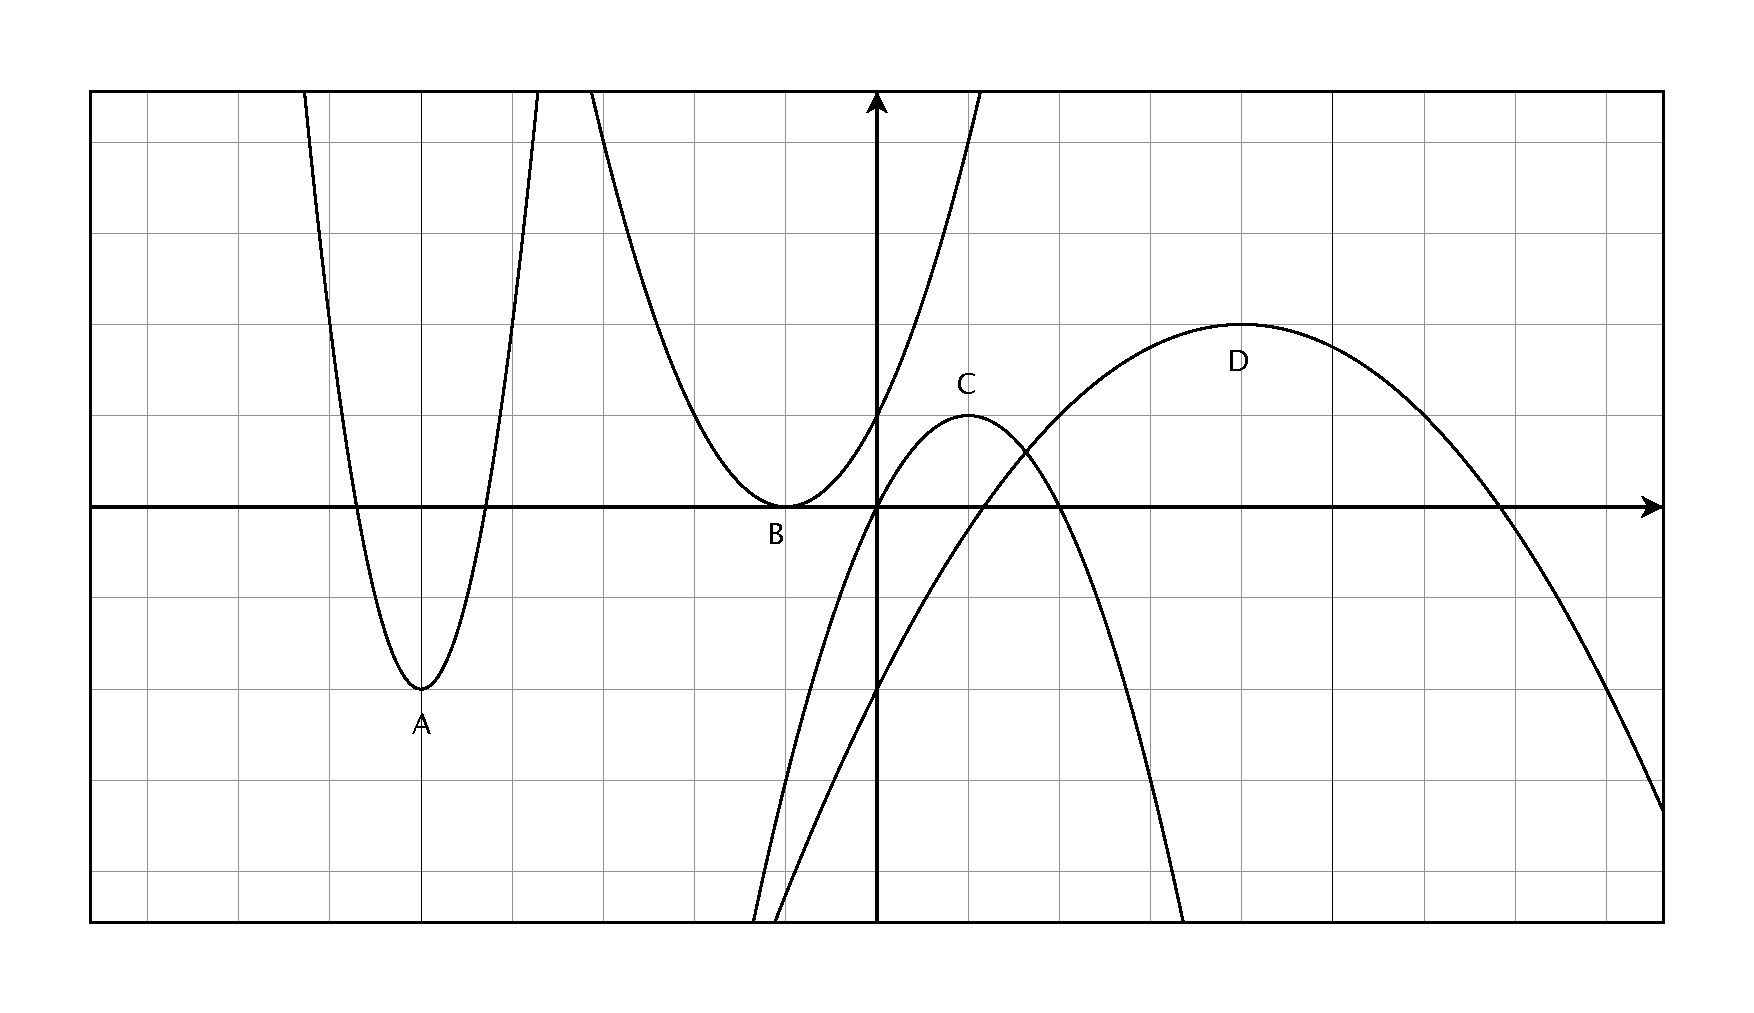
\includegraphics[scale=.3]{problem_7.eps}
%   \caption*{Problem 7}
% \end{figure}

% \begin{tabular}{cc}
% \toprule
% period & amplitude \\
% \midrule
%   $\pi$ & $2$ \\
% \bottomrule
% \end{tabular}

\title{Math 141 \\ Chapter Two Study Guide}
\date{February 27, 2013}

\begin{document}

\maketitle
\tableofcontents

\section{Introduction}

This study guide summarizes what I think are the important points from Chapter 2.

Good ways to practice are:
\begin{itemize*}
  \item Do the problems in the {\em Chapter Two Review} on pages 233-236.
  \item Do the chapter 2 practice test on 237-238.
  \item Review this study guide and make sure you know how to do all the types of problems.
\end{itemize*}

\section{Section 2.1--Functions}

\subsection{Notes}

A function is a rule for transforming numbers in the {\em domain} to numbers in the {\em range}.  Each number in the
domain is matched with exactly one number in the range.

You can tell if a graph is a graph of a function with the {\em Vertical Line Test}.  If you can draw a vertical line
which hits the graph of the function more than once, than you don't have a function.

The {\em domain} of a function is all the numbers that are allowed as inputs.  Sometimes the domain is explicitly
specified but more often it's implied.  Any number that would make the denominator zero or make a square root negative,
for example, is excluded from the domain.

There are four ways to specify a function:
\begin{itemize*}
  \item verbally with a description in words: ``add two''.
  \item algebraically with a formula: $f(x) = x + 2$.
  \item with a graph 
  \item with a table of values
\end{itemize*}

A ``piecewise defined'' function is a combination of more than one function with a rule which tells you when to use each
one.  For example:
\[
  f(x) = 
    \begin{cases}
      3x        & \text{if } x < 0 \\
      x + 1     & \text{if } 0 \leq x \leq 2 \\
      (x - 2)^2 & \text{if } x > 2 \\
    \end{cases}
\]

If $x$ is negative, you use $f(x) = 3x$, if $x$ is between zero and 2, you use $f(x) = x + 1$ and if $x$ is bigger than
two, you use $f(x) = (x - 2)^2$.

\subsection{Problems}
You should be able to:
\begin{itemize*}
  \item Evaluate a function at a number expression (problems 13-20)
  \item Evaluate piecewise defined functions (problems 21-24)
  \item Know the difference between things like $f(x + 2)$ and $f(x) + 2$ (problems 25-28)
  \item Find the domain, watching out for values that would make the expression inside a square root negative or a
    denominator zero (problems 37-58).
  \item Find functions which represent problems stated in words (problems 59-73).
\end{itemize*}

\section{Section 2.2--Basic Graphing}

\subsection{Notes}

You can graph a line in the form $y = mx + b$ using its slope and y-intercept.

The simplest way to graph a function that isn't a line is to select some x values and plug them in to get the
corresponding y values.

You can use the {\em Vertical Line Test} to determine if a graph is the graph of a function.

\subsection{Problems}
\begin{itemize*}
  \item Graph a line using the slope and intercept (problems 1-5);
  \item Graph functions by selecting some $x$ values and evaluating them in the function (1-22, 38-50);
  \item Find the domain and range of a function from its graph (problem 23-24);
  \item Use the vertical line test to determine if a graph is the graph of a function (problems 55-60);
  \item Determine if an equation is a function (problems 61-72);
  \item Use functions and graphs in applications (problems 83-90).
\end{itemize*}

\section{Section 2.3--Increasing/Decreasing/Average Rate of Change}

\subsection{Notes}

A function is {\em increasing} over an interval if it is constantly getting bigger.  More formally, $f(x)$ is increasing
on $[a, b]$ if for any $x_1$ and $x_2$ in $[a, b]$, if $x_2 > x_1$, then $f(x_2) > f(x_1)$.

The definition of a {\em decreasing} function is similar.  $f(x)$ is decreasing on $[a, b]$ if for any $x_1$ and $x_2$
in $[a, b]$, if $x_2 > x_1$, then $f(x_2) < f(x_1)$.

The average rate of change for a function on an interval is the change in the value of the function divided by the size
of the interval.  As an equation, the average rate of change for $f$ on $[a, b]$ is:
\[
  a = \frac{f(b) - f(a)}{b - a}
\]

\subsection{Problems}
\begin{itemize*}
  \item Find regions where a function is increasing/decreasing from its graph (problems 1-4);
  \item Find the average rate of change for a function from its graph (problems 13-16);
  \item Find the average rate of change for a function from its equation (problems 17-28);
  \item Use rate of change and increasing/decreasing ideas in applications (problems 31-39);
\end{itemize*}

\section{Section 2.4--Graph Transformations}

\subsection{Notes}

The simplest way to graph a function is to select some x values and plug them in to get the corresponding y values.
This can be a lot of work, however.  In addition, no matter how many points you select, you might not end up choosing
interesting ones, so you could end up with an inaccurate picture of the function.  

If you can write your function as a modification of a function you already know how to graph, then you can apply these
rules to get the graph of your function.  Suppose the function you want to graph is $f(x)$ and it is similar to
$g(x)$.

\begin{itemize*}
  \item If $f(x) = g(x) \pm c$, the graph of $f(x)$ is the graph of $g(x)$ shifted up/down by $c$.
  %\item If $f(x) = g(x) - c$, the graph of $f(x)$ is the graph of $g(x)$ shifted down by $c$.
  \item If $f(x) = g(x \pm c)$, the graph of $f(x)$ is the graph of $g(x)$ shifted left/right by $c$.
  % \item If $f(x) = g(x - c)$, the graph of $f(x)$ is the graph of $g(x)$ shifted right by $c$.
  \item If $f(x) = c \cdot g(x)$, the graph of $f(x)$ is the graph of $g(x)$ scaled vertically by $c$.  
  \item If $f(x) = g(c \cdot x)$, the graph of $f(x)$ is the graph of $g(x)$ scaled horizontally by $c$.  
\end{itemize*}

\subsection{Problems}
\begin{itemize*}
  \item Describe the effect of adding, subtracting, or multiplying by a constant on a graph (problems 1-10, 23-54).
  \item Go backwards from a graph to an equation (problems 11-22)
  \item Know the definition of even and odd functions and be able to identify the graph of an even/odd function
    (problems 55-58)
  \item Know how to tell if a function is even/odd from its equation (problems 61-68)
\end{itemize*}

\section{Section 2.5--Quadratic Functions, Maxima and Minima}

\subsection{Notes}

The {\em Standard Form} for a quadratic function is:
\[
  f(x) = a(x - h)^2 + k
\]

This is a useful form to have the equation in because you can read some useful things from the graph:
\begin{itemize}
  \item The {\em vertex} is at the point $(h, k)$.

  \item If $a > 0$
    \begin{itemize*}
      \item The parabola opens up.
      \item The minimum value of $k$ occurs when $x = h$.
      \item The range is $[k, \infty)$.
    \end{itemize*}

  \item If $a < 0$
    \begin{itemize*}
      \item The parabola opens down.
      \item The maximum value of $k$ occurs when $x = h$.
      \item The range is $(-\infty, k]$.
    \end{itemize*}
\end{itemize}

You can put a quadratic function in standard form by {\em completing the square}.

The easiest way to find the minimum or maximum (depending on the sign of the $x^2$ coefficient) is to use:
\begin{align*}
  x_{min/max} &= \frac{-b}{2a} \\
  y_{min/max} &= f(x_{min/max}) \\
\end{align*}

A {\em local minimum/maximum} is a point where $f(x)$ is larger/smaller than any of its immediate neighbors, but not
necessarily larger/smaller than all other values in the range.  For quadratic functions, any local minimum/maximum is
also a global minimum/maximum.

\subsection{Problems}

\begin{itemize*}
  \item Find the vertex, min/max, and range of a quadratic function from its graph (problems 1-4)

  \item Put the equation for a quadratic function in standard form and find the min/max and vertex from the equation ins
    standard form (problems 5-28)

  \item Use $x_{min/max} = \frac{-b}{2a}$ to find the minimum/maximum value and range (problems 29-38, 41-44)

  \item Find the equation for a parabola given the vertex and a point (problems 39-40).

  \item Find local minimums and maximums from graphs (problems 47-50).

  \item Use minimum/maximum techniques in applications (problems 59-65).

\end{itemize*}

\section{Section 2.6--Modeling with Functions}

\subsection{Notes}

You can often use functions to model real-world minimization/maximization problems.  The usual steps are:
\begin{itemize}
  \item Define some variables to represent the quantities in the problem and translate the problem into one or more equations.

  \item If you have two equations and two variables, solve one of the equations for the variable you
    want to eliminate and plug the result into the other equation.

  \item Find the minimum/maximum in the resulting quadratic equation using $x_{min/max} = \frac{-b}{2a}$.

  \item Plug $x_{min/max}$ into the original equation to find the actual minimum or maximum value.
\end{itemize}

\subsection{Problems}
You should know how to do all the problems from section 2.6.  Typical types of problems are:
\begin{itemize*}
  \item Maximize volume given a shape (sphere, box, etc.) and surface area
  \item Maximize area given a shape and fixed perimeter (farmer and pens, etc.)
  \item Find minimum distance between two moving objects.
  \item Minimize the product of two numbers, given a fixed sum.
\end{itemize*}

\section{Section 2.7--Combining Functions}

\subsection{Notes}

You can create new functions by adding, subtracting, multiplying or dividing other functions.  

For everything but division, the domain of the new function is the intersection of the two original domains.  For
division, the new domain is the intersection of of the two original domains with any values that make the new
denominator zero also excluded.

You still have to preserve the original domains, even if they wouldn't cause a problem in the new function.  For
example, suppose you have:
\begin{align*}
  f(x) &= \frac{1}{x} \\
  g(x) &= x^2 \\
  (fg)(x) &= \frac{1}{x} \cdot x^2 = x \\
\end{align*}

The domain of $(fg)(x)$ is still $x \neq 0$ because this was the domain of $f$.

Another interesting way to combine functions is to chain them together.  This is called {\em composition}, and the two
notations are: $f(g(x))$ and $(f \circ g)(x)$.  You apply $g$ to $x$ and then apply $f$ to the result.  The domain is
all $x$ values in the domain of $g$ where $g(x)$ is in the domain of $f$.

\subsection{Problems}

\begin{itemize*}
  \item Add, subtract, multiply, and divide two functions to get new functions and find the domain for the new functions
    (problems 1-10)

  \item Create a new function by composing two other functions (problems 17-44)

  \item Express a complicated function as the composition of two or more simpler functions (problems 45-54)

  \item Understand applications of combining functions (problems 55-62).
\end{itemize*}

\section{Section 2.8--One-to-One Functions and Inverses}

\subsection{Notes}

A function is ``one-to-one'' if each value in the range can only come from one value in the domain.  

$f(x) = x^2$ is not one-to-one because every value in the range except for 0 could have come from either a positive or
negative value in the domain.  On the other hand, $f(x) = x^3$ is one-to-one.

An easy test to see if a function is one-to-one is the {\em Horizontal Line Test}.  If you can draw a horizontal
line that intersects the graph of the function at more than one spot, then the function is not one-to-one.

One-to-one functions are interesting because they have {\em inverses}.  An inverse function, $f^{-1}(x)$ undoes whatever
the original function did.  In other words:
\begin{align*}
  f(f^{-1}(x)) &= x \\
  f^{-1}(f(x)) &= x \\
\end{align*}

To find the inverse:
\begin{itemize*}
  \item Write the function as $y = \text{ expression }$
  \item Solve for $x$ in terms of $y$.
  \item Replace $y$ with $x$ in the result.
  \item Check that you didn't make an algebra mistake by verifying that $f(f^{-1}(x)) = f^{-1}(f(x)) = x$
\end{itemize*}

Sometimes you can restrict the domain of a function that isn't one-to-one to get a one-to-one function that has an
inverse.  For example, if you restrict the domain of $f(x) = x^2$ to $x \geq 0$, then $f(x)$ has an inverse: 
$f^{-1}(x) = \sqrt{x}$.

The inverse of a function can also be obtained by reflecting the original function in the line $y = x$, but sometimes
this is easier said than actually drawn.

\subsection{Problems}

\begin{itemize*}
  \item Determine if a function is one-to-one (problems 1-16)

  \item Demonstrate that two functions are inverses of each other (problems 21-30)

  \item Find inverse functions (problems 31-50)

  \item Know how to restrict the domain of a function to make it one-to-one (problems 65-68).

  \item Understand applications of inverse functions (problems 71-79).
\end{itemize*}

\end{document}

